\subsection{Grasper Design}

\subsubsection{Latch Mechanism}

The chosen design for the grasper consists of a rotating clasp, driven by a servo motor. A rendering of the design
is shown in Fig. \ref{fig:clasp-design}, and the OpenSCAD source used to create it can be found in appendix \ref{app:grasper-scad}.
The \texttt{BOSL2} library \cite{belfryscad_bosl2_nodate} was used to create the gear components.

\begin{figure}[H]
    \centering
    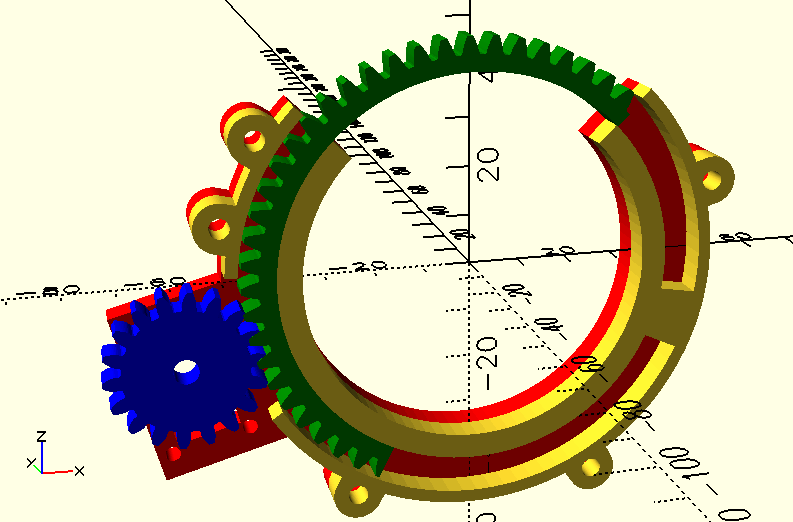
\includegraphics[width=\textwidth]{sections/methods/grasper-render.png}
    \caption{Rendering of the proposed grasping device. The backplate shown in red is meant to hold 
    a servo, which drives the gear shown in blue. The green, toothed semicircle is driven by the blue gear to
    open and close the grasper, and bears the weight of the device and drone once closed over a perch. The
    yellow part supports and guides the green latch. Note that in the real device there is a third plate closing 
    the front of the device, but it is not shown here so that the gear and latch mechanism are visible.}
    \label{fig:clasp-design}
\end{figure}

The device used here has an inner radius of 35mm, which results in it being able to accept a perch of up to 
50mm diameter. The outer radius of the device is 50mm. The latch component (green object in Fig. \ref{fig:clasp-design})
has a radial width of 7.4mm.

\subsubsection{Controller}

A Raspberry Pi Compute Module 4 was used to control the servos on the grasper device. To avoid 
complicating the design with limit switches to detect open and closed states, an Adafuit 
ADS1015 analog-digital converter was used to measure the current drawn by each servo.
The current measurement is used to detect when the servo has stalled, indicating 
that the limits of travel are reached and the latch has either fully opened or closed.

The schematic of the servo control module can be seen in appendix \ref{app:schematics},
Fig. \ref{fig:clasp-ctl}. The schematic showing the compute module and its interface to the
servo controller can be seen in appendix \ref{app:schematics},
Fig. \ref{fig:cpu-module}.


\subsection{Grasper Verification}

\subsubsection{Holding Capacity}

The specifications of popular commercial drones were assessed to determine common weights of drones,
to determine weight that this drone might need to support.
Table \ref{tab:drone-weights} shows the assessed models and their weights.

\begin{table}[H]
    \centering
    \caption{Specified Weight of Various Commercial Drones}
    \begin{tabular}{| c || c |}
        \hline
        {Make \& Model} & Weight (g) \\
        \hline
        DJI Mavic Pro & 734 \\
        DJI Mavic 3 Pro & 958 \\
        DJI Mavic 3 Enterprise & 920 \\
        DJI Mavic Mini & 249 \\
        Parrot ANAFI USA & 500 \\
        FLIR SIRAS & 3100 \\
        Autel EVO Max 4T & 1640 \\
        DJI Matrice 30 & 3770 \\
        \hline
    \end{tabular}
    \label{tab:drone-weights}
\end{table}

There appear to be a few classes of drones represented:
\begin{itemize}
    \item Sub 500g lightweight drones
    \item Sub 1kg medium drones
    \item Heavy weight 1.5 kg + drones
\end{itemize}

This device was designed to hold a drone of up to 500g, plus 31.58 N
of dynamic load, for a total static load of 3.72 kg.

The dynamic load is to allow for force introduced by motion of the perch, such as a swaying tree branch.
Assuming that the drone is perched in a tree and subject to sinusoidal motion, its maximum acceleration is estimated at $63.17 m/s^2$ 
based on data provided by Kamimura et al. (0.4 m max displacement with a frequency of 2 Hz) \cite{kamimura_energy_2024}.  
The referenced study did use only Japanese Cedar, which may not
be representative of all trees. However, similar data for other species could not be found.

The first reason for targeting the lowest weight group is that the low weight is far more
manageable for the device to hold. The other reasons are cost and risk. The medium and heavy drones tend to be significantly 
more expensive, and are used to carry higher quality cameras. Leaving a drone perched in a tree or other location leaves
it exposed to risk of damage, which makes using a larger drone for this particularly unappealing to the drone's owner.

The achieved holding capacity of the device was achieved with the following test process:
\begin{enumerate}
    \item The grasper was closed around a test perch, suspended above the ground.
    \item A bag was attached to the underside of the grasper, close to the center of its baseplate in the x-y plane.
    \item Weights were added to the bag incrementally, with a 10-minute period between each addition.
    \item Once the device breaks before the 10-minute period has expired after the most recent addition, the holding capacity
        is determined to be the load weight at the previous successful weight addition.
\end{enumerate}

To avoid damaging the electronic components when the device failed, all except the servos were removed for the duration of this test. 
The device is capable of remaining attached without power to the servos, and the weight of the removed electronics was removed from the
final weight at the end of the test. The results are summarized in Section \ref{sec:results:capacity}


\subsubsection{Weight}

Table \ref{tab:payload} shows rated payload for various drones, which were used 
The rated payload was calculated as the rated maximum total takeoff weight minus the drones specified weight. 
The DJI Mavic products had no maximum takeoff weight aside from the products weight, so no maximum payload is listed for them. 

\begin{table}[H]
    \centering
    \caption{Rated Payload of Various Commercial Drones}
    \begin{tabular}{| c || c |}
        \hline
        {Make \& Model} & Payload (g) \\
        \hline
        DJI Mavic Pro & None Rated \\
        DJI Mavic 3 Pro & None Rated \\
        DJI Mavic 3 Enterprise & 130 \\
        DJI Mavic Mini & None Rated \\
        Parrot ANAFI USA & 144 \\
        FLIR SIRAS & 3100 \\
        Autel EVO Max 4T & 379 \\
        DJI Matrice 30 & 299 \\
        \hline
    \end{tabular}
    \label{tab:payload}
\end{table}

In the sub 500g category, only the Parrot ANAFI has a rated payload. This will be assumed as a reasonable estimate for the
payload capacity of similarly sized drones. In order to leave some margin for safety, and possible additional task-specific
modifications, this devices weight shall be no more than 33\% of that capacity, or 47.5g. This target weight will also 
provide improvements over similar existing designs \cite{chi_optimized_2014,nguyen_passively_2019}.

The overall weight and weight of individual components of the device were measured and recorded in table \ref{tab:weights}.

\subsubsection{Repeatability}

To verify that the proposed design can open and close reliably, the opening and closing process was manually 
repeated 30 times. Each time after closing the grasper or opening it again, the device was 
visually inspected to ensure that:
\begin{itemize}
    \item The latch had not become stuck on any other part of the device, causing stall detection to trigger
        prematurely and prevent successful opening or closing.
    \item The latch had not failed to engage with the servo, preventing it from moving.
\end{itemize}

If opening or closing was not successful, then that test was marked as a failure, and the specific reason recorded.
The success rate and failure causes are shown in Section \ref{sec:results:repeatability}.